


\begin{figure}[t]%h!
    \centering
    \begin{subfigure}{.47\textwidth}
        \centering
        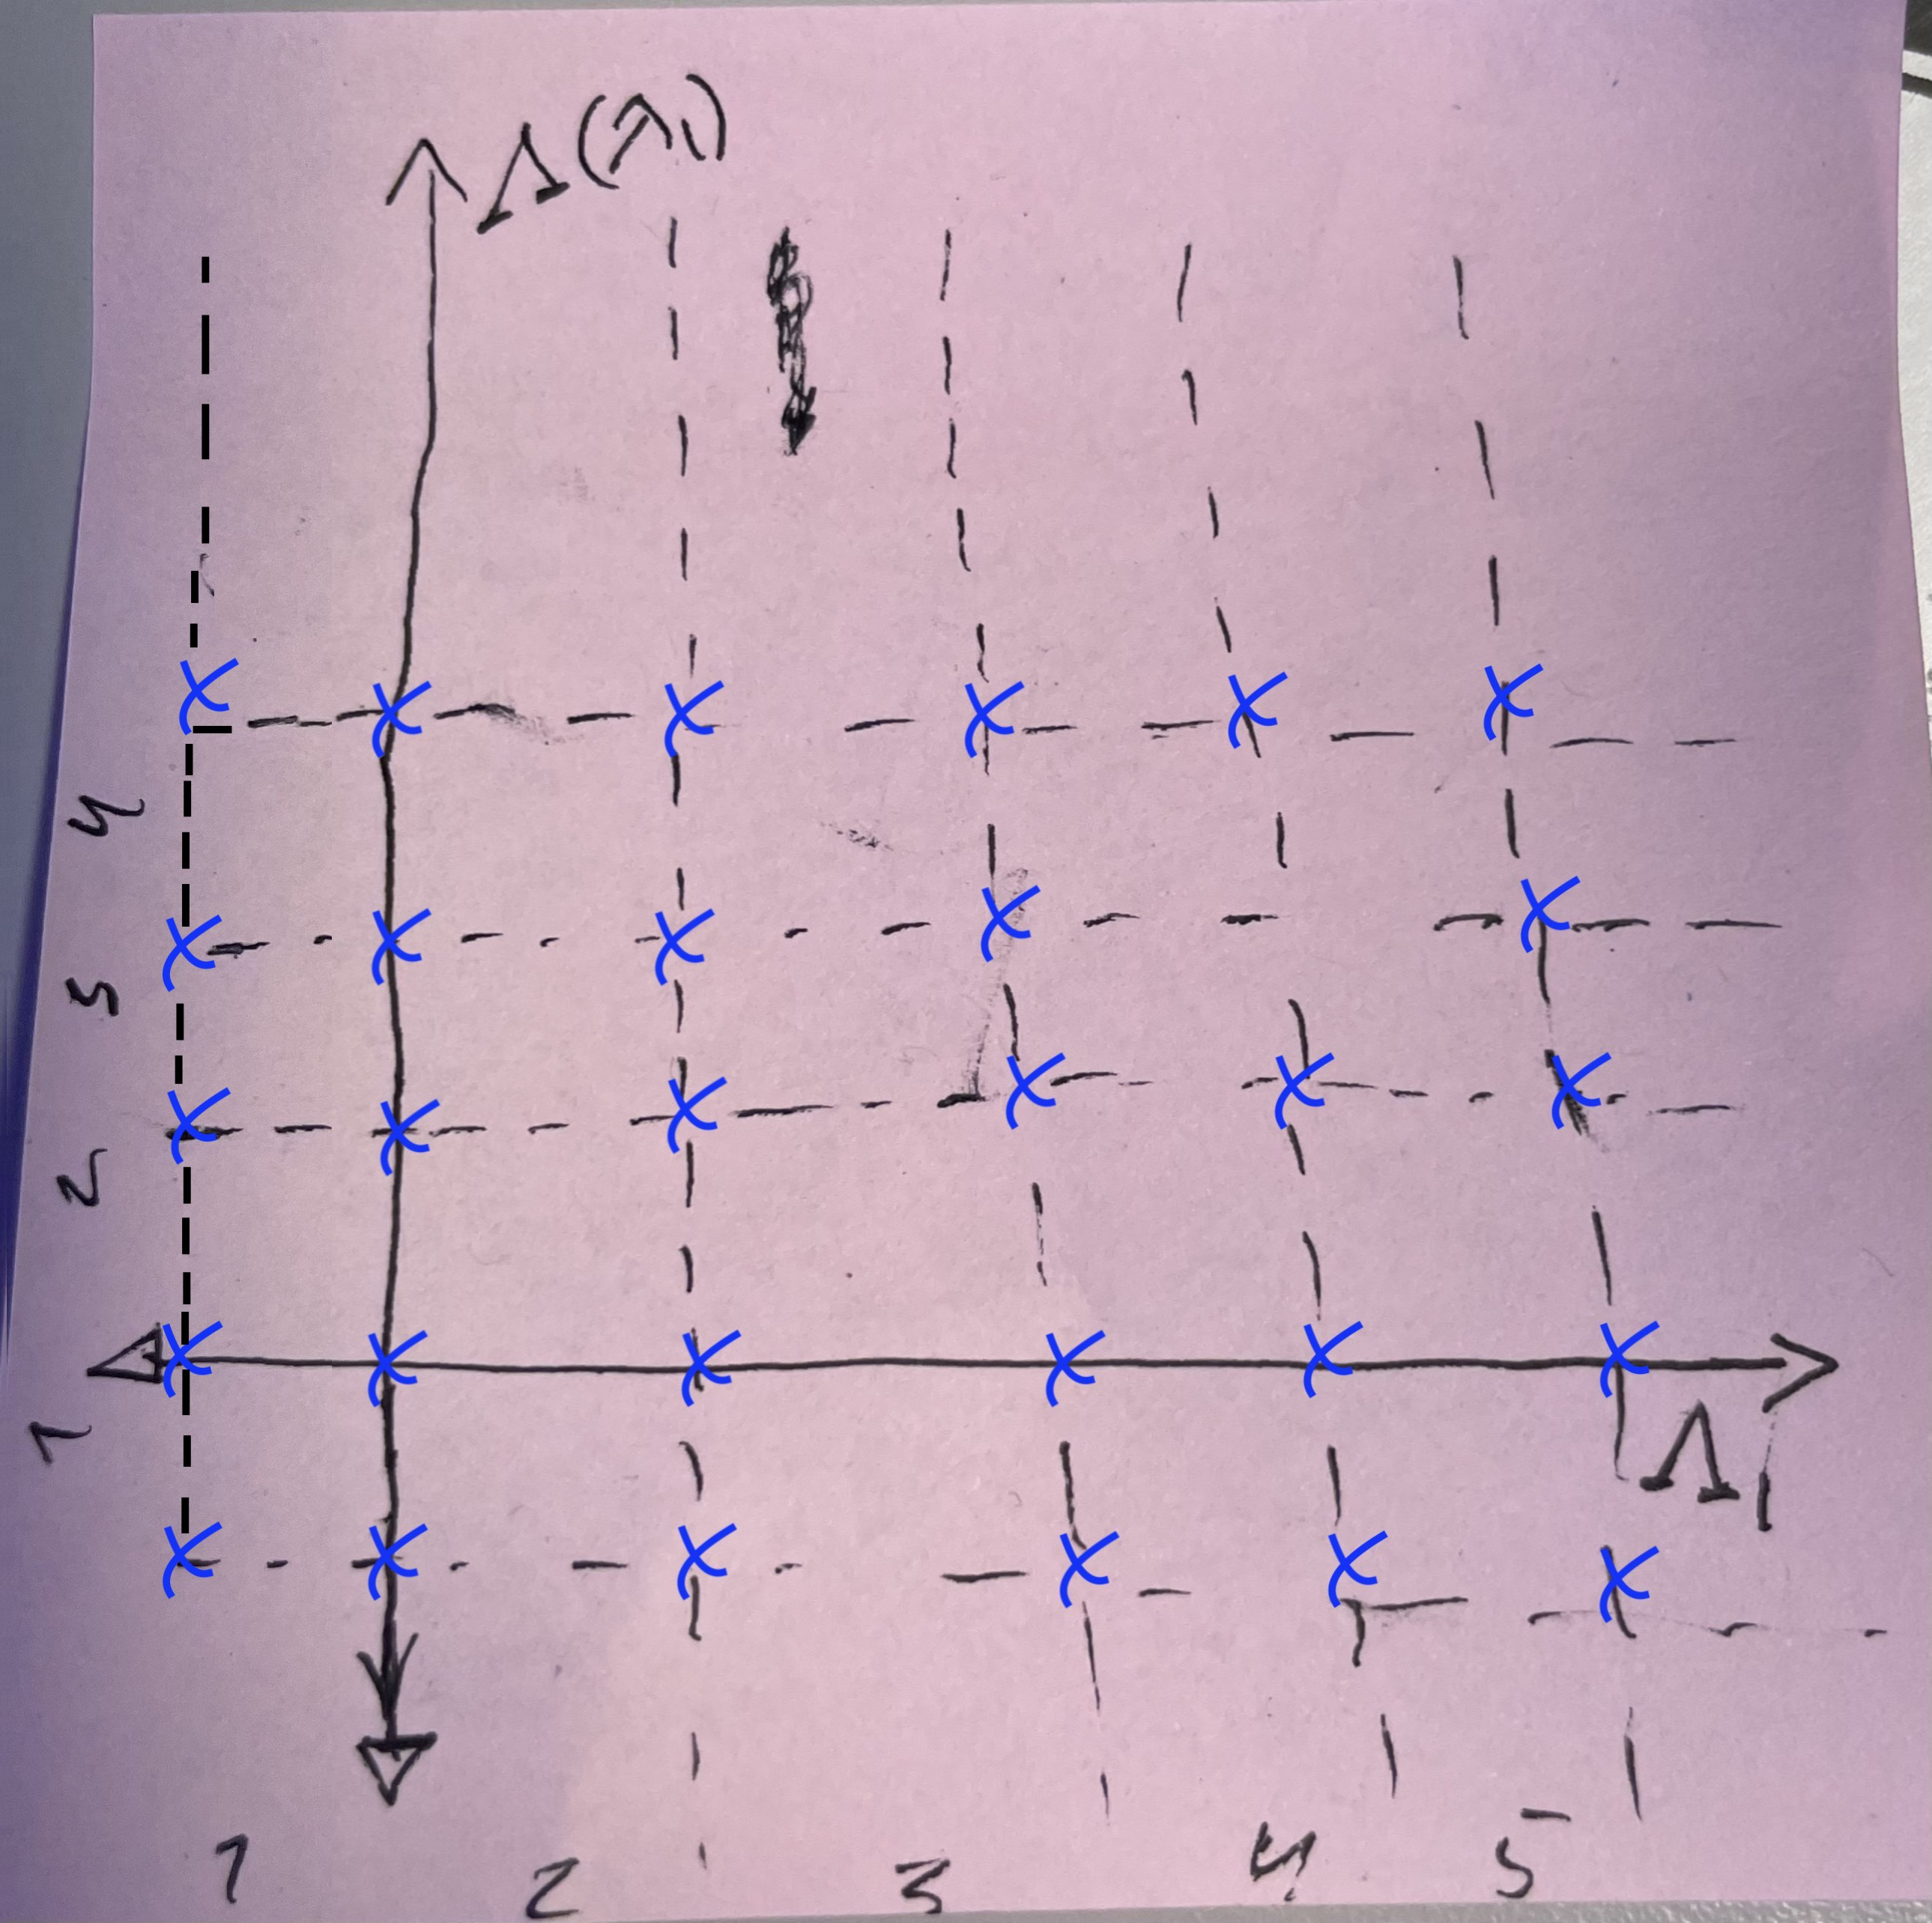
\includegraphics[width=0.9\linewidth]{spec_no_shift.jpg}
        \caption{Lattice spectra}
        \label{fig:lattice_spectra}
    \end{subfigure}\quad
    \begin{subfigure}{.47\textwidth}
        \centering
        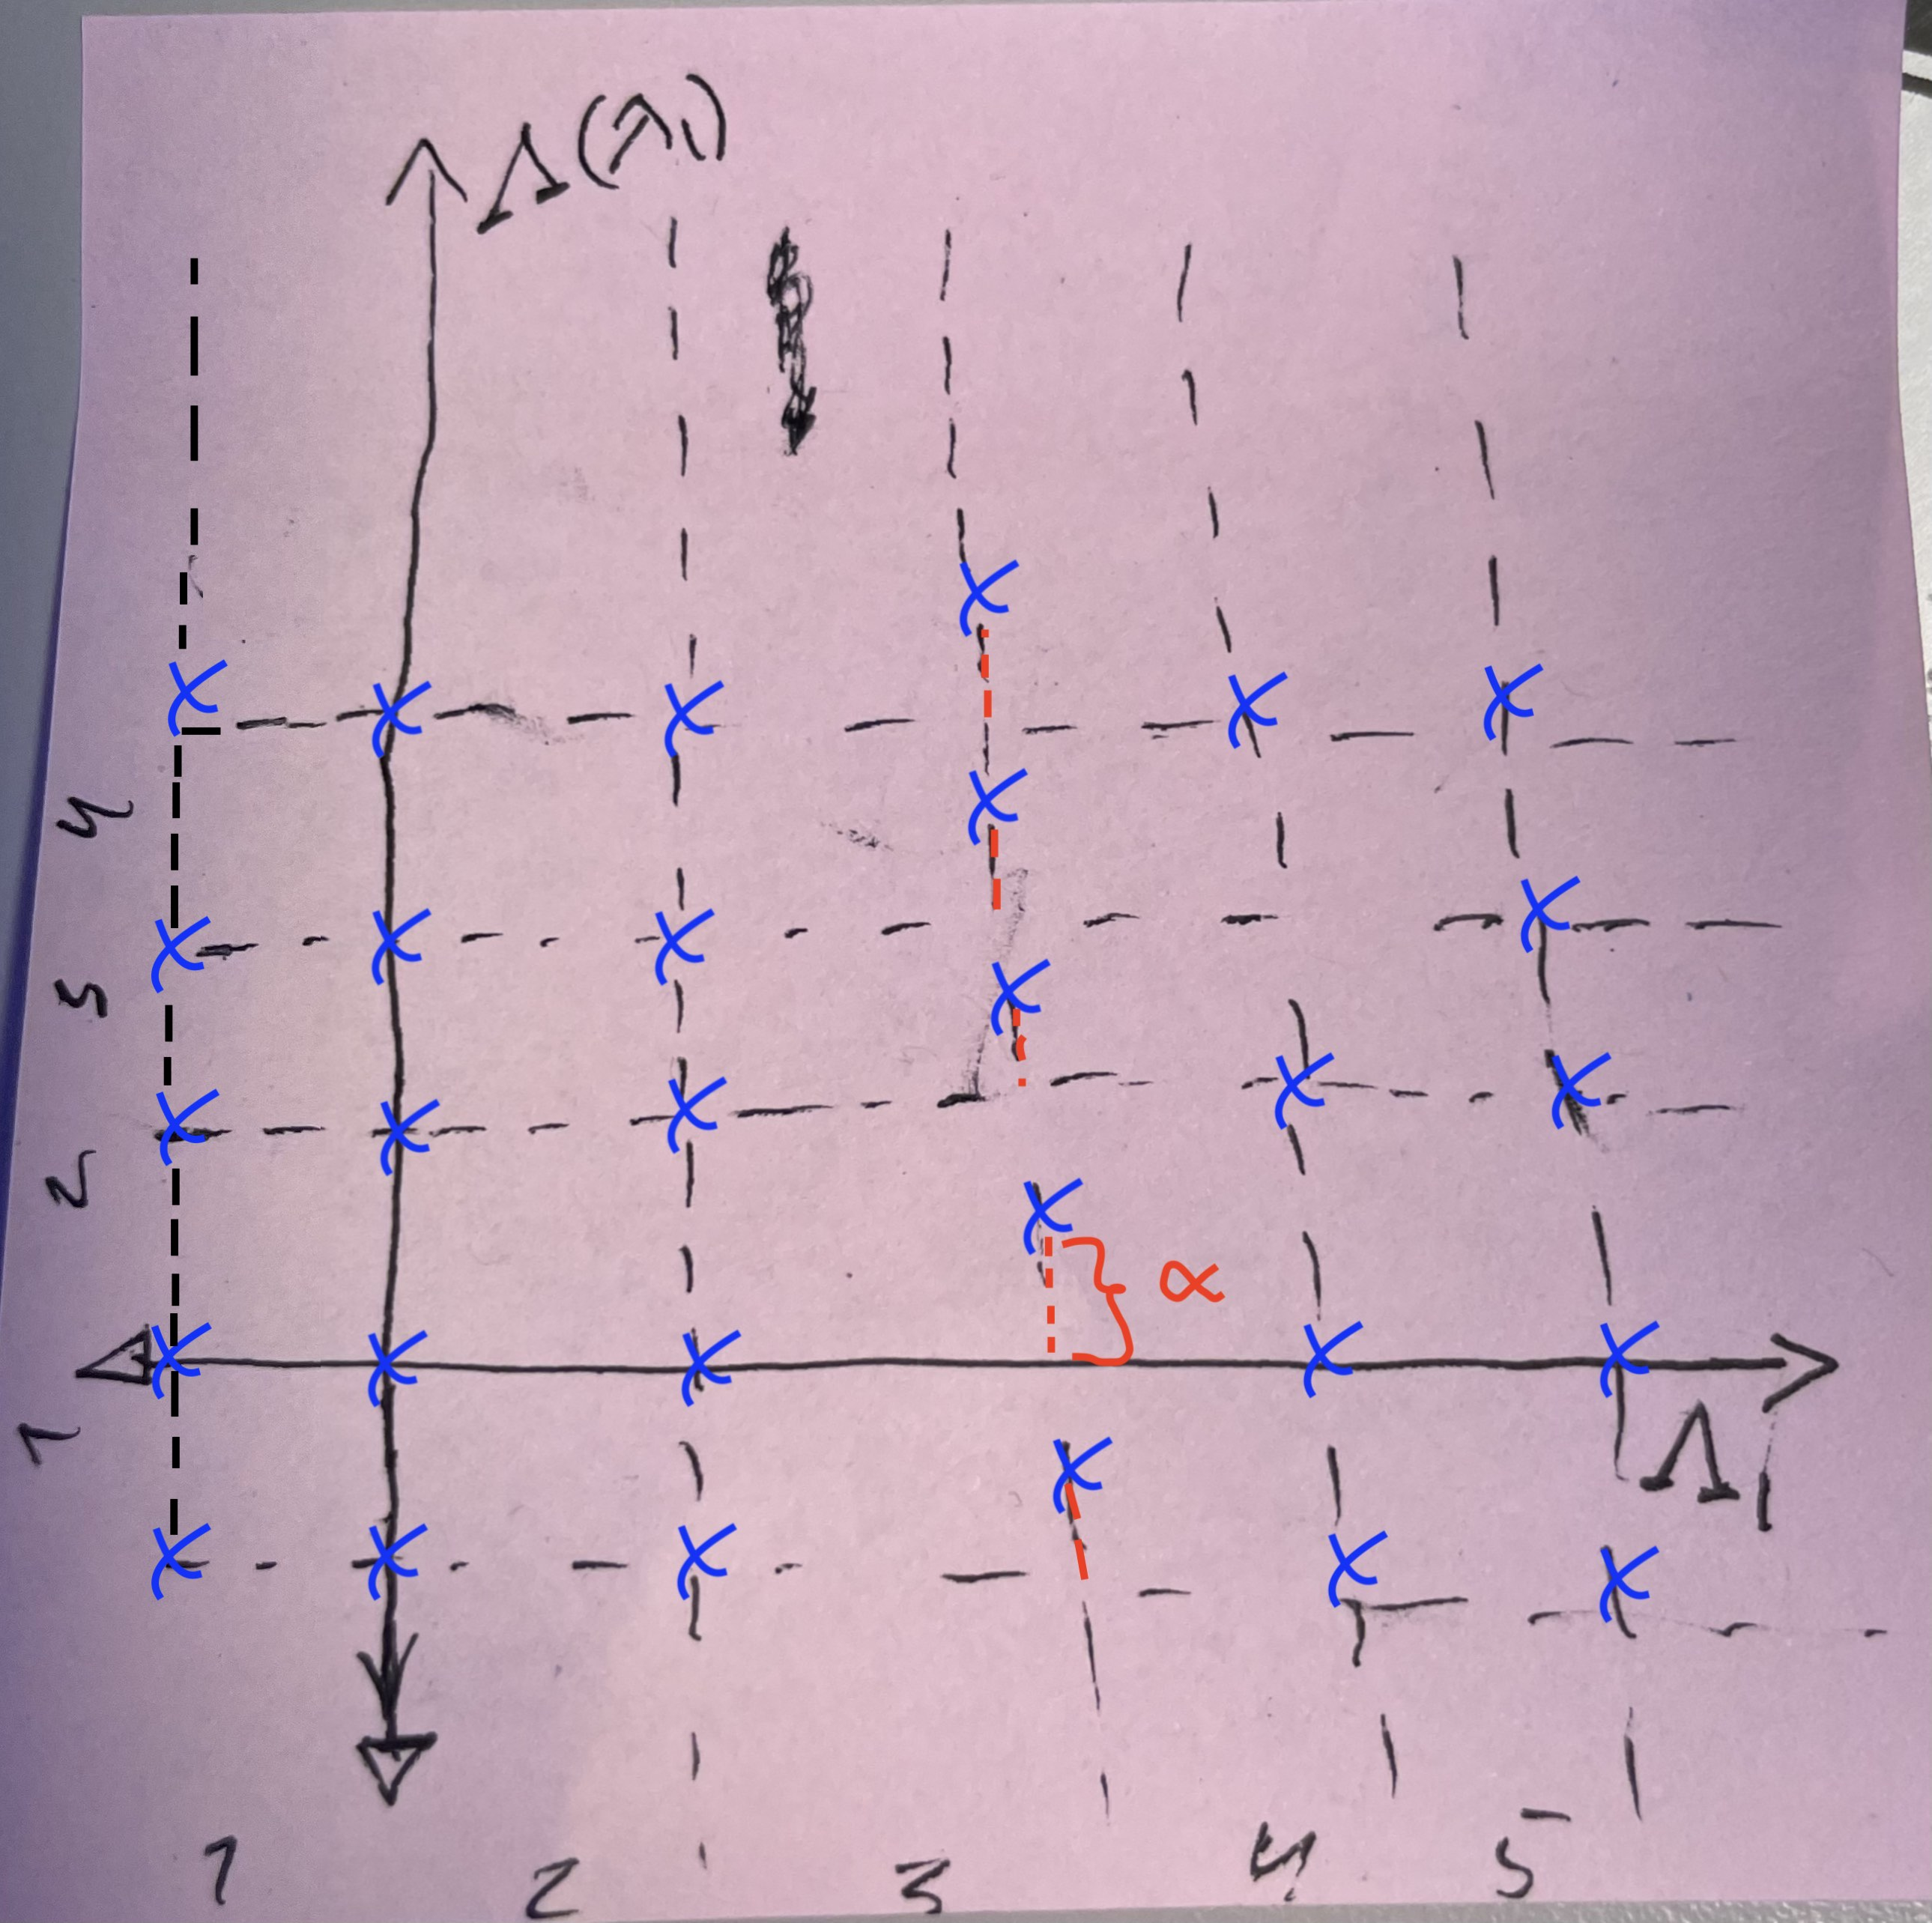
\includegraphics[width=0.9\linewidth]{spec_single_shift.jpg}
        \caption{Single shift vertical}
        \label{fig:single_shift_vertical}
    \end{subfigure}\\
    \begin{subfigure}{.47\textwidth}
        \centering
        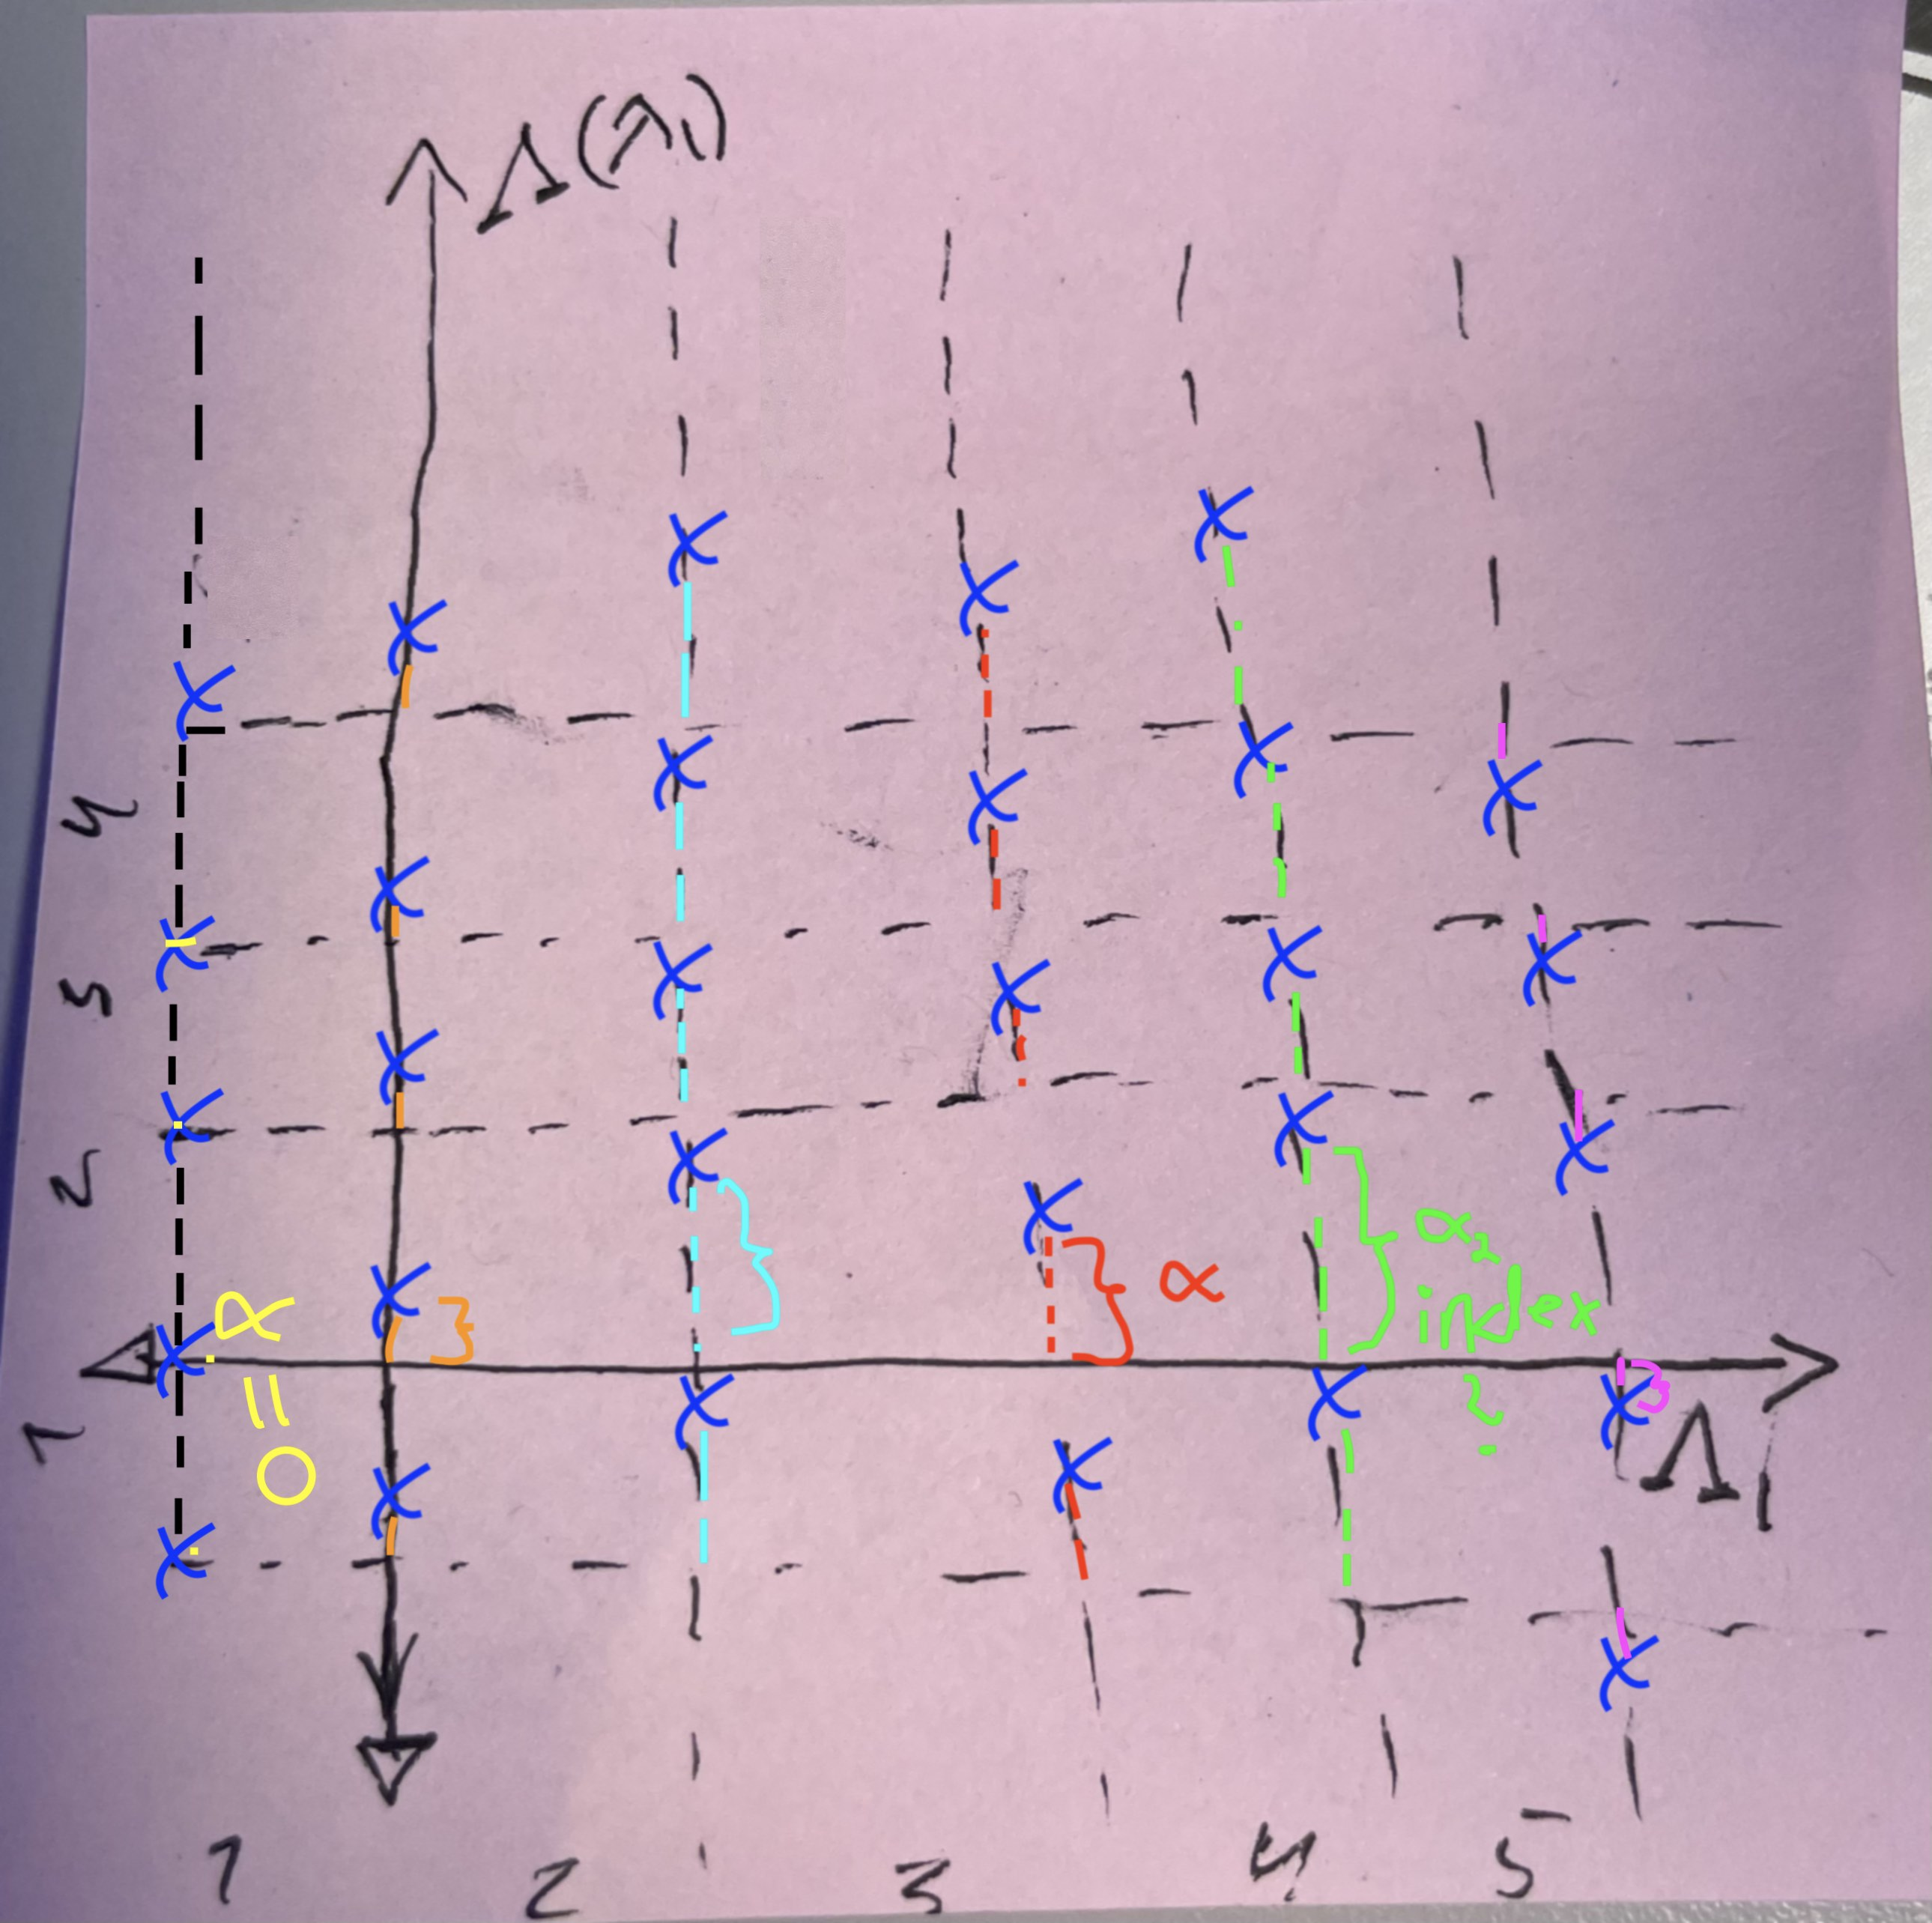
\includegraphics[width=0.9\linewidth]{multiple_shift_left_zero.jpg}
        \caption{Multiple individual shifts vertical}
        \label{fig:multiple_shift_vertical}
    \end{subfigure}\quad
    \begin{subfigure}{.47\textwidth}
        \centering
        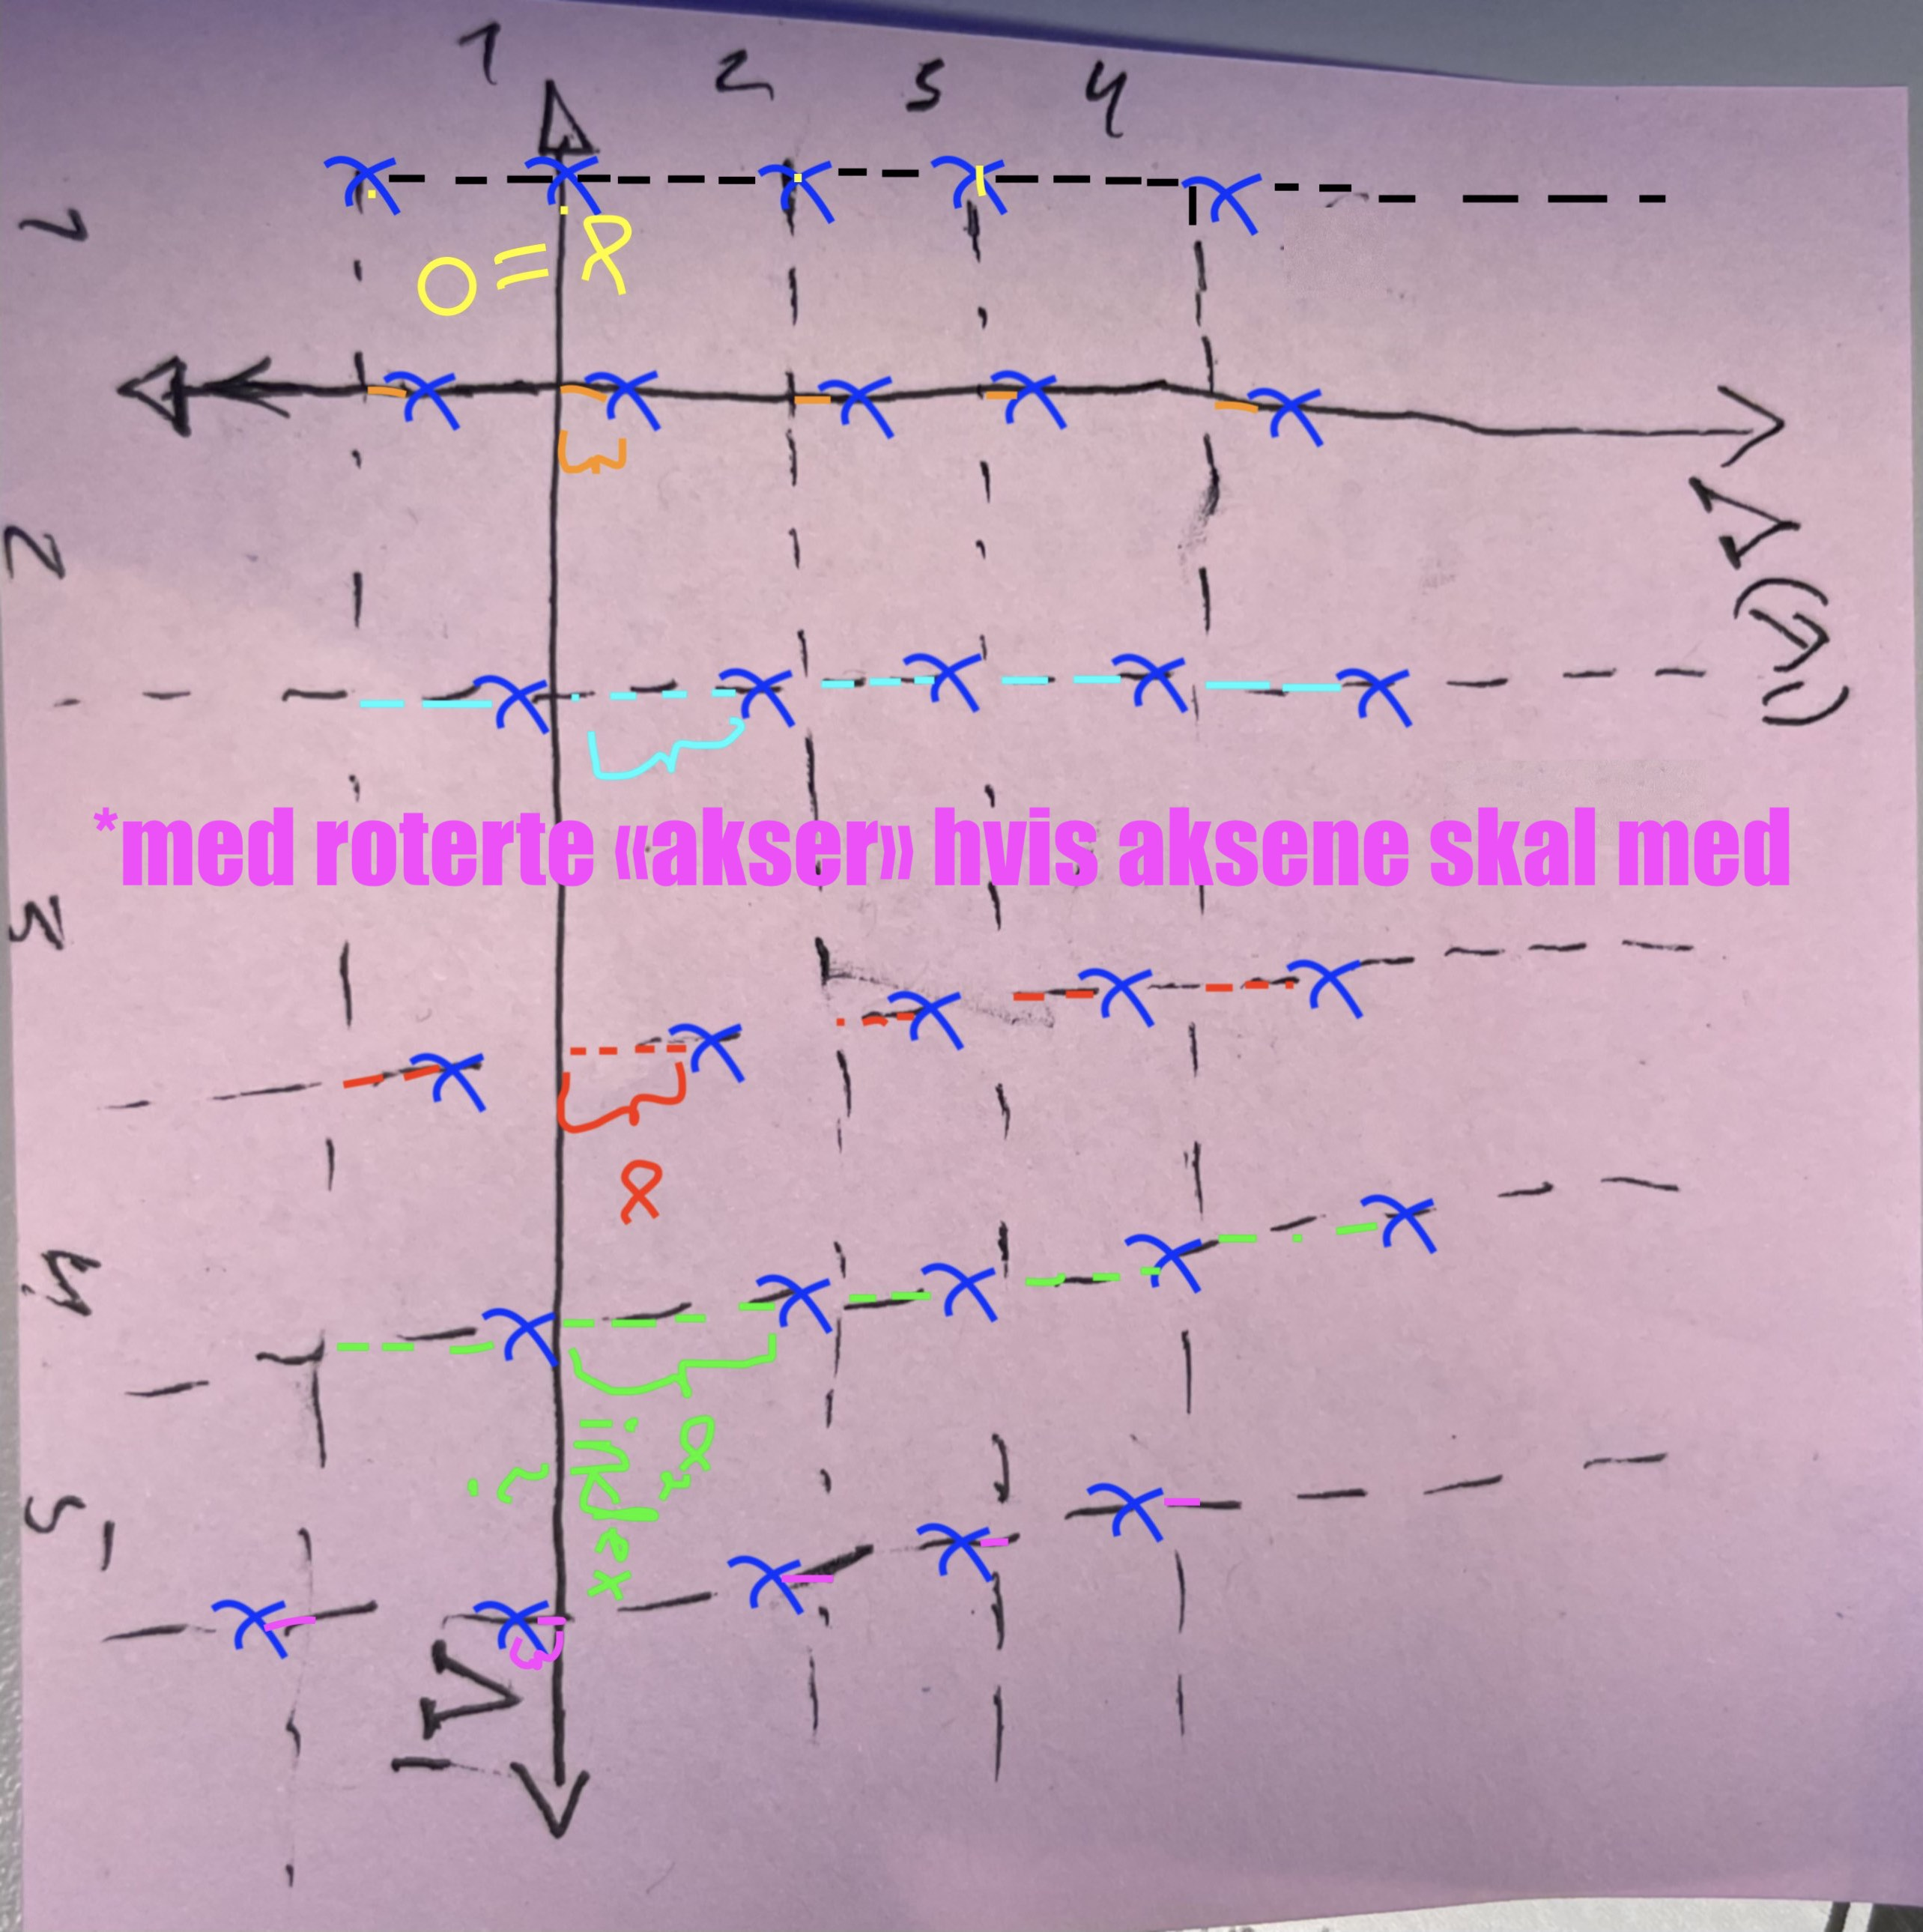
\includegraphics[width=0.9\linewidth]{multiple_shift_left_zero_horizontal.jpg}
        \caption{Multiple individual shifts horizontal}
        \label{fig:multiple_shift_horizontal}
    \end{subfigure}
    \caption{Illustration of the following pair of spectral pairs. In \labelcref{fig:lattice_spectra} we have $\brac{I,\Z}$ and $\brac{I,\lambfunc}$.  In \labelcref{fig:single_shift_vertical} we have $\brac{I,\Z}$ and $\brac{I,\lambfunc}$, where $\lambfunc$ is given by \labelcref{eq:single_shift_func}. In \labelcref{fig:multiple_shift_vertical} we have $\brac{I,\Z}$ and $\brac{I,\lambfunc}$, where $\lambfunc$ is given by \labelcref{eq:multiple_shit_func}. In \labelcref{fig:multiple_shift_horizontal} we have $\brac{I,\Z+0.4}$ and $\brac{I,\lambfunc}$, where $\lambfunc$ is given by \labelcref{eq:multiple_shit_func}.}
    \label{fig:spectra_figures}
\end{figure}
